\documentclass[a4paper,12pt,twoside]{memoir}

% Castellano
\usepackage[spanish,es-tabla]{babel}
\selectlanguage{spanish}
\usepackage[utf8]{inputenc}
\usepackage[T1]{fontenc}
\usepackage{lmodern} % Scalable font
\usepackage{microtype}
\usepackage{placeins}

\RequirePackage{booktabs}
\RequirePackage[table]{xcolor}
\RequirePackage{xtab}
\RequirePackage{multirow}

% Links
\PassOptionsToPackage{hyphens}{url}\usepackage[colorlinks]{hyperref}
\hypersetup{
	allcolors = {red}
}

% Ecuaciones
\usepackage{amsmath}

% Rutas de fichero / paquete
\newcommand{\ruta}[1]{{\sffamily #1}}

% Párrafos
\nonzeroparskip

% Huérfanas y viudas
\widowpenalty100000
\clubpenalty100000

\let\tmp\oddsidemargin
\let\oddsidemargin\evensidemargin
\let\evensidemargin\tmp
\reversemarginpar

% Imágenes

% Comando para insertar una imagen en un lugar concreto.
% Los parámetros son:
% 1 --> Ruta absoluta/relativa de la figura
% 2 --> Texto a pie de figura
% 3 --> Tamaño en tanto por uno relativo al ancho de página
\usepackage{graphicx}

\newcommand{\imagen}[3]{
	\begin{figure}[!h]
		\centering
		\includegraphics[width=#3\textwidth]{#1}
		\caption{#2}\label{fig:#1}
	\end{figure}
	\FloatBarrier
}







\graphicspath{ {./img/} }

% Capítulos
\chapterstyle{bianchi}
\newcommand{\capitulo}[2]{
	\setcounter{chapter}{#1}
	\setcounter{section}{0}
	\setcounter{figure}{0}
	\setcounter{table}{0}
	\chapter*{#2}
	\addcontentsline{toc}{chapter}{#2}
	\markboth{#2}{#2}
}

% Apéndices
\renewcommand{\appendixname}{Apéndice}
\renewcommand*\cftappendixname{\appendixname}

\newcommand{\apendice}[1]{
	%\renewcommand{\thechapter}{A}
	\chapter{#1}
}

\renewcommand*\cftappendixname{\appendixname\ }

% Formato de portada

\makeatletter
\usepackage{xcolor}
\newcommand{\tutor}[1]{\def\@tutor{#1}}
\newcommand{\tutorb}[1]{\def\@tutorb{#1}}

\newcommand{\course}[1]{\def\@course{#1}}
\definecolor{cpardoBox}{HTML}{E6E6FF}
\def\maketitle{
  \null
  \thispagestyle{empty}
  % Cabecera ----------------
\begin{center}
  \noindent\includegraphics[width=\textwidth]{cabeceraSalud}\vspace{1.5cm}%
\end{center}
  
  % Título proyecto y escudo salud ----------------
  \begin{center}
    \begin{minipage}[c][1.5cm][c]{.20\textwidth}
        \includegraphics[width=\textwidth]{escudoSalud.pdf}
    \end{minipage}
  \end{center}
  
  \begin{center}
    \colorbox{cpardoBox}{%
        \begin{minipage}{.8\textwidth}
          \vspace{.5cm}\Large
          \begin{center}
          \textbf{TFG del Grado en Ingeniería de la Salud}\vspace{.6cm}\\
          \textbf{\LARGE\@title{}}
          \end{center}
          \vspace{.2cm}
        \end{minipage}
    }%
  \end{center}
  
    % Datos de alumno, curso y tutores ------------------
  \begin{center}%
  {%
    \noindent\LARGE
    Presentado por \@author{}\\ 
    en Universidad de Burgos\\
    \vspace{0.5cm}
    \noindent\Large
    \@date{}\\
    \vspace{0.5cm}
    %Tutor: \@tutor{}\\ % comenta el que no corresponda
    Tutores: \@tutor{} -- \@tutorb{}\\
  }%
  \end{center}%
  \null
  \cleardoublepage
  }
\makeatother

\newcommand{\nombre}{Rocío Alonso las Heras}
\newcommand{\nombreTutor}{Antonio Jesús Canepa Oneto} 
\newcommand{\nombreTutorb}{Estefanía Rivas Navas} 
\newcommand{\dni}{71188698H} 

% Datos de portada
\title{ASMR Sleep. Aplicación de recomendación y análisis de vídeos destinada a pacientes con Insomnio de Conciliación.}
\author{\nombre}
\tutor{\nombreTutor}
\tutorb{\nombreTutorb}
\date{\today}


\begin{document}

\maketitle


\newpage\null\thispagestyle{empty}\newpage

%%%%%%%%%%%%%%%%%%%%%%%%%%%%%%%%%%%%%%%%%%%%%%%%%%%%%%%%%%%%%%%%%%%%%%%%%%%%%%%%%%%%%%%%
\thispagestyle{empty}


\noindent\includegraphics[width=\textwidth]{cabeceraSalud}\vspace{1cm}

\noindent D. \nombreTutor, profesor y director del Área de Lenguajes y Sistemas Informáticos del Departamento de Ingeniería Informática y Dña. Estefanía Rivas Navas, médico en el Hospital Universitario de Burgos, en el departamento de neurofisiología clínica y en la unidad del sueño.

\noindent Expone:

\noindent Que la alumna Dña. \nombre, con DNI \dni, ha realizado el Trabajo final de Grado en Ingeniería de la Salud titulado título del trabajo. 

\noindent Y que dicho trabajo ha sido realizado por la alumna bajo la dirección del que suscribe, en virtud de lo cual se autoriza su presentación y defensa.

\begin{center} %\large
En Burgos, {\large \today}
\end{center}

\vfill\vfill\vfill

% Author and supervisor
\begin{minipage}{0.45\textwidth}
\begin{flushleft} %\large
Vº. Bº. del Tutor:\\[2cm]
D. \nombreTutor
\end{flushleft}
\end{minipage}
\hfill
\begin{minipage}{0.45\textwidth}
\begin{flushleft} %\large
Vº. Bº. del Tutor:\\[2cm]
D. \nombreTutorb
\end{flushleft}
\end{minipage}
\hfill

\vfill

% para casos con solo un tutor comentar lo anterior
% y descomentar lo siguiente
%Vº. Bº. del Tutor:\\[2cm]
%D. nombre tutor


\newpage\null\thispagestyle{empty}\newpage

\frontmatter
    \begin{center}
       \vspace*{5cm}
        \textit{A mi madre y a mis abuelas, por estudiar y por no haber podido hacerlo, gracias por acompañarme hasta aquí.}
        \vfill 
    \end{center}



\frontmatter

% Abstract en castellano
\renewcommand*\abstractname{Resumen}
\begin{abstract}
Debido al aumento reciente en las problemáticas relacionadas con el sueño y los hábitos de descanso, que afectan negativamente la calidad de vida y el bienestar general de las personas, surge la necesidad de desarrollar herramientas de apoyo y ayuda que puedan mitigar estos problemas y promover mejores hábitos. Este trabajo de fin de grado propone el desarrollo de una aplicación de recomendación de vídeos de ASMR, utilizando el lenguaje de programación R y la estructura de la aplicación, Shiny para crear una herramienta interactiva y personalizada que ayude a los usuarios a encontrar contenido de ASMR adecuado a sus necesidades individuales. Este proyecto no solo aborda una problemática de salud pública cada vez más relevante, sino que también aprovecha el potencial de la tecnología y el contenido digital para ofrecer soluciones innovadoras y accesibles.
\end{abstract}

\renewcommand*\abstractname{Descriptores}
\begin{abstract}
Respuesta Sensorial Meridiana Autónoma, ASMR, insomnio, redes sociales, R, RStudio, Shiny, YouTube Data, API, intervenciones tecnológicas, recomendación de vídeos, calidad del sueño.
\end{abstract}

\clearpage

% Abstract en inglés
\renewcommand*\abstractname{Abstract}
\begin{abstract}
Due to the recent increase in sleep-related problems and rest habits, which negatively affect people's quality of life and general well-being, there is a need to develop support and assistance tools that can mitigate these issues and promote better habits. This final degree project proposes the development of an ASMR video recommendation application, using the R programming language and the Shiny application framework to create an interactive and personalized tool that helps users find ASMR content suited to their individual needs. This project not only addresses an increasingly relevant public health issue but also leverages the potential of technology and digital content to offer innovative and accessible solutions.
\end{abstract}

\renewcommand*\abstractname{Keywords}
\begin{abstract}
Autonomous Sensory Meridian Response, ASMR, social media, R, RStudio, Shiny, YouTube Data, API, technological interventions, video recommendations, sleep quality.
\end{abstract}

\clearpage

% Indices
\tableofcontents

\clearpage

\listoffigures

\clearpage

\listoftables
\clearpage


\mainmatter
\include{./tex/1_introduccion}
\include{./tex/2_objetivos}
\include{./tex/3_teoricos}
\include{./tex/4_metodologia}
\include{./tex/5_resultados}
\include{./tex/6_conclusiones}
\include{./tex/7_lineas_futuras}

\chapter{Introducción}

El presente Trabajo de Fin de Grado se centra en la creación de una aplicación de búsqueda y recomendación de vídeos de ASMR, diseñada específicamente para pacientes con insomnio de conciliación. Este proyecto, realizado en el contexto del grado en Ingeniería de la Salud, surge de la necesidad de explorar nuevas formas de abordar el problema del insomnio mediante el uso de tecnología y terapias no convencionales.\\*\\*
En la actualidad, la influencia de las redes sociales en las conductas y hábitos de la población es innegable \cite{levenson2016}. Entre las diversas tendencias que han surgido en este contexto, el fenómeno del \textit{Autonomous Sensory Meridian Response},o Respuesta Sensorial Meridiana Autónoma en castellano (ASMR), ha ganado popularidad en los últimos años. El ASMR se refiere a una experiencia sensorial placentera, caracterizada por una sensación de hormigueo en el cuero cabelludo y el cuerpo, que se desencadena por estímulos visuales o auditivos específicos, como susurros, sonidos suaves o movimientos lentos. \\*

El interés en el ASMR ha crecido considerablemente en las plataformas de redes sociales \cite{jerez-2023}, donde miles de videos están dedicados a este fenómeno y la supuesta ayuda que proporciona a aquellos usuarios que los consumen para relajarse y dormir. Sin embargo, a pesar de su popularidad, el ASMR sigue siendo una tendencia relativamente poco estudiada, especialmente en lo que respecta a su potencial para abordar problemas de salud como el insomnio de conciliación.\\*

El sueño juega un papel fundamental en la salud y el bienestar general de las personas \cite{nelson2021}. Durante el sueño, el cuerpo se recupera y se regenera, mientras que el cerebro procesa y consolida la información adquirida durante el día. Sin embargo, en la sociedad moderna, cada vez más personas experimentan dificultades para conciliar el sueño debido al estrés, el uso excesivo de dispositivos electrónicos y los cambios en el estilo de vida. La prevalencia del insomnio ha aumentado significativamente en los últimos años, lo que ha llevado a una mayor conciencia sobre la importancia de abordar los problemas relacionados con el sueño. En este contexto, surge la necesidad de explorar nuevas estrategias y terapias para mejorar la calidad del sueño y promover el bienestar general de las personas.\\*

La aplicación desarrollada se basa en Shiny, lo que permite crear una interfaz simple e intuitiva para que los usuarios puedan encontrar y explorar vídeos de ASMR. Además de proporcionar funciones de búsqueda y recomendación, la aplicación también incluye información educativa sobre qué es el ASMR y cómo puede beneficiar a los pacientes con problemas de sueño.\\*

Para alimentar la base de datos de vídeos de ASMR, se utiliza la API de YouTube Data, que proporciona acceso a una amplia variedad de contenido relacionado con el ASMR en la plataforma de YouTube. Además, la aplicación permite a los usuarios crear registros de calidad del sueño, lo que les permite realizar un seguimiento de su progreso y evaluar el impacto de los vídeos de ASMR en su sueño.\\*

En resumen, este Trabajo de Fin de Grado busca explorar el potencial del ASMR como una intervención terapéutica para el insomnio de conciliación, a través del desarrollo de una aplicación innovadora y fácil de usar que aprovecha la tecnología y la información disponible en las redes sociales.
\chapter{Objetivos del proyecto}

\section{Objetivos Generales}
\begin{itemize}
    \item Explorar el potencial clínico del fenómeno ASMR como medida auxiliar en tratamiento de patologías relacionadas con el sueño a través del desarrollo de una aplicación de recomendación de videos 
    \item Describir formalmente de manera completa el fenómeno ASMR, incluyendo una revisión del estado del arte de publicaciones sobre el tema
    \item Caracterizar las conductas saludables de sueño y el insomnio

\end{itemize}

\section{Objetivos Técnicos}
\begin{itemize}
    \item Proponer una solución tecnológica a pacientes con insomnio de conciliación relacionado con el uso de ASMR y redes sociales, en concreto YouTube
    \item Desarrollar una aplicación Shiny en R para la recomendación de vídeos ASMR
    \item Crear en la aplicación dos roles diferenciados, usuario y administrador, con funciones específicas para cada uno de ellos
    \item Implementar una base ded datos local mediante un sistema gestor de bases de datos como SQLite
    \item  Programar una consulta a través de una interfaz de programación de aplicaciones (API, por sus sigles en Inglés) del servicio API YouTube Data, para obtener datos en tiempo real
    \item Diseñar el frontend de la aplicación mediante CSS
    \item Plantear posibles medidas de mejora que puedan implementarse en futuras versiones de la aplicación
    
\end{itemize}

\section{Objetivos Personales}
\begin{itemize}
    \item Unificar los conocimientos de la rama sanitaria con los relacionados con la rama tecnológica obtenidos durante el grado
    \item Proponer una solución innovadora que integre en el tratamiento clínico de una patología una herramienta poco empleada aún pero con un gran potencial como son las redes sociales
    \item Desarrollar una aplicación de manera autónoma, utilizando para ellos una variedad de lenguajes
    \item Obtener una mejor comprensión de los recursos disponibles para el desarrollo de tecnologías, como manuales, APIs proporcionadas por las empresas, foros online y herramientas de inteligencia artificial
    \item Realizar una contribución al mundo del estudio formal del fenómeno ASMR
\end{itemize}

\chapter{Conceptos teóricos}
    \text Los fundamentos teóricos que sustentan este trabajo se enmarcan en dos disciplinas clave: la información médica y la tecnología.  \\*\\*
    \section{Teoría clínica} En primer lugar, la sección clínica del trabajo se dedica a proporcionar una descripción exhaustiva del concepto general de sueño y descanso, abordando posteriormente los diversos trastornos del sueño, con un enfoque particular en el insomnio de conciliación. Este análisis incluirá una revisión de la literatura existente, los mecanismos fisiológicos y psicológicos implicados, así como las estrategias diagnósticas y terapéuticas utilizadas en la práctica clínica. \\*\\*En lo que respecta al componente tecnológico, se ofrecerá una descripción detallada de la red social YouTube, la plataforma sobre la cual se basarán las búsquedas y el análisis. Se explorará el uso de YouTube, su crecimiento exponencial a lo largo de los años, su relevancia en la difusión de información y su potencial aplicación en el ámbito clínico. Este análisis incluirá estadísticas de uso, características de la audiencia, y ejemplos de contenido relacionado con la salud y el bienestar. Además, se discutirá cómo YouTube puede ser una herramienta útil para los profesionales de la salud en la educación y el apoyo a los pacientes, y se evaluará su impacto en la promoción de hábitos saludables y en la concienciación sobre trastornos del sueño como el insomnio de conciliación.

    \subsection {El sueño}
    \begin{figure}
    \centering
    \includegraphics[width=1\textwidth]{imagenes/mctrastornos.png}
    \caption{Mapa conceptual trastornos del sueño. Elaboración propia}
    \label{fig:enter-label}
\end{figure}
    \text Para comprender las implicaciones del insomnio es necesario dar unas nociones básicas sobre el sueño, que se considera normal y recomendable en este proceso, y a que se debe su importancia en la salud. \\*\\*El sueño es un proceso biológico fundamental para el ser humano que tiene varios propósitos diferentes, que incluyen el descanso para la restauración física, la consolidación de la memoria, la regulación emocional, la conservación de la energía, la regulación hormonal y la reposición de neurotransmisores \cite{assefa2015}. \\*\\*Las recomendaciones de horas de sueño varían según la edad, estas se encuentran en 14-17 horas para recién nacidos, 11-15 horas para niños menores de 3 años, 10-13 horas para niños en edad preescolar, 9-11 horas para niños en edad escolar, 8-10 para adolescentes, 7-9 para jóvenes adultos y 7-8 horas para adultos mayores \cite{hirshkowitz2015}, llegando en edades superiores a 60 años a ser la recomendación de 6,5 horas \cite{ferre2020}. \\*\\*Pese a que las recomendaciones generales se han hecho tradicionalmente sin discriminación de género, basadas en estudios hechos en población masculina o mixta, algunos estudios más recientes comienzan a sugerir que las necesidades de las mujeres podrían diferir de estas recomendaciones debido a sus patrones hormonales, tanto a largo plazo como durante las diferentes fases del ciclo menstrual \cite{andersen2023}.\\*\\*Los efectos adversos de una calidad de sueño deficiente de este son objeto constante de estudio, y actualmente se relacionan con múltiples patologías diferentes como la diabetes, distintas enfermedades cardiovasculares, depresión, ansiedad, obesidad, ataques al corazón, accidentes cerebrovasculares y distintos tipos de cáncer \cite{nelson2021,ma2016}.

    \subsection {Principales trastornos del sueño}
    \text La 5ª edición del Manual de Diagnóstico y Estadístico de los Trastornos Mentales publicado por la Asociación Estadounidense de Psiquiatría (APA), el DSM-5, clasifica entre los principales trastornos del sueño \cite{guadamuz2022}: 

    \begin{itemize}
    \item Insomnio (en el que se profundizará a continuación)
    \item Hipersomnia: Trastorno del sueño que se caracteriza por una somnolencia extrema durante el día, lo que conduce a una necesidad excesiva de dormir y dificultad para despertarse por completo, incluso después de un período prolongado de sueño.
    \item Narcolepsia: Trastorno neurológico crónico caracterizado por la excesiva somnolencia diurna y episodios repentinos de sueño durante el día.
    \item Trastornos del sueño relacionados con la respiración: En este apartado pueden incluirse múltiples trastornos distintos en los que no se profundizará, pero entre ellos se encuentran la apnea o hipopnea obstructiva del sueño, apnea central del sueño, hipoventilación relacionada con el sueño, entre otros.
    \item Trastorno del ritmo circadiano: Implica alteraciones en el ciclo natural de sueño-vigilia del cuerpo, causando dificultades para conciliar el sueño, despertares tempranos o tardíos y un patrón de sueño desalineado con los horarios sociales convencionales.
    \item Parasomnia: Conjunto de trastornos del sueño que implican comportamientos o experiencias anormales durante el sueño, como sonambulismo, terrores nocturnos, somniloquia (hablar durante el sueño) o comportamientos violentos durante el sueño REM.
    
    \subsection{El insomnio}
    \text El insomnio es el trastorno del sueño que presenta la mayor prevalencia en adultos a nivel mundial, las estimaciones no son exactas, pero calculan que entre un 10 y un 15\% de la población general mundial lo padecen \cite{Contreras2021}. Este trastorno puede presentar diferentes manifestaciones, desde dificultades a la hora de conciliar el sueño, mantener la continuidad del mismo o conseguir una calidad de sueño adecuada que permita que el descanso se lleve a cabo de manera correcta \cite{kaur2023}. \\*\\* La prevalencia de este trastorno varía por países, en Europa en 2023 los datos estimaron que esta patología se presentaba de manera crónica en 1 de cada 10 adultos \cite{kaur2023}, otros países tienen una incidencia de este trastorno notablemente más alta, como por ejemplo Estados Unidos (2023) donde se estima que un tercio de los adultos de la población general lo sufre \cite{kaur2023}.\\*\\*La Sociedad Española de Neurología (SEN) estimaba en un comunicado de prensa de 2024, con motivo del Día  Mundial del Sueño y Día Europeo de la Narcolepsia, una prevalencia general de casos puntuales de insomnio de entre el 20 y el 48\%. Los casos de insomnio crónico se sitúan en un 10\% \cite{perez2024}. \\*\\* En este comunicado sugieren que los tres aspectos más importantes a tener en cuenta a la hora de evaluar la calidad del sueño son: la duración, la continuidad y la profundidad.\\*\\*Esta patología puede clasificarse de diferentes maneras, dependiendo al criterio que se atienda, en cuanto a la naturaleza del insomnio, este puede clasificarse en \cite{ferre2020}: 
\begin{itemize}
    \item Insomnio de conciliación: Se refiere a la dificultad para conciliar el sueño al principio de la noche, lo que resulta en una demora prolongada para quedarse dormido.
    \item Insomnio de mantenimiento: Se caracteriza por dificultades para mantener el sueño durante la noche, lo que provoca despertares frecuentes y dificultad para volver a conciliar el sueño.
    \item Insomnio de despertar precoz: Es similar al insomnio de mantenimiento, dificultad para mantener el sueño durante la noche, con despertares tempranos y la incapacidad de volver a dormirse, lo que resulta en un despertar final anticipado en la mañana.
    \item Insomnio mixto o absoluto: Se utiliza esta terminología para hablar de aquel tipo de insomnio que incluye distintos tipos de insomnio de los anteriormente mencionados.
\end{itemize}

    \text El insomnio también puede clasificarse según el tiempo durante el que se presenta, los  tres tipos son insomnio transitorio o agudo, a corto plazo o subagudo y a largo plazo o crónico. El insomnio se considera crónico, se diagnostica y recibe tratamiento cuando los episodios se presentan al menos 3 veces por semana durante 3 meses o más \cite{diagnosisNHLBI}.
En la figura 3.1 se encuentra un resumen visual de lo explicado en este apartado.
    \subsection{Diagnóstico del insomnio}
    \begin{figure}
    \centering
    \includegraphics[width=1\textwidth]{imagenes/venninsomnio.png}
    \caption{Diagrama de Venn Conceptos Básicos Insomnio}
    \label{fig:enter-label}
\end{figure}
    \text La sospecha de la presencia de insomnio surge en las consultas, generalmente de atención primaria, durante la anamnesis. No todos los pacientes describen síntomas graves de insomnio, por lo que es necesario realizar preguntas para clasificar el problema concreto de cada paciente para valorar si es necesario derivarlos a especialistas o pueden hacer un diagnóstico, tratamiento y seguimiento adecuado los profesionales de atención primaria, es por ello que se publican guías para el diagnóstico.\\*\\*Algunos de los signos de alarma que manifiesta el insomnio que han de tenerse en cuenta para su diagnóstico diferencial son la presentación de somnolencia diurna, presencia de ronquido o apneas, presencia de siestas de más de 60 minutos de duración, patadas o agitación nocturna, presencia del insomnio después de 3 meses de tratamiento médico y valores de ferritina por debajo de 75ng/ml \cite{ferre2020}. Las principales preguntas a las que el paciente debe responder para poder realizar un diagnóstico diferencial de insomnio se agrupan en 5 categorías:
    \begin{itemize}
        \item Hábitos de sueño: Horarios, número de veces que se despierta, tiempo desvelado, siestas durante el día etc.
        \item Síntomas nocturnos:  ronquidos, apneas, sonambulismo, mioclonías, nicturia (necesidad de orinar durante la noche), enuresis (pérdidas accidentales de orina) etc.
        \item Síntomas al despertar: Cefaleas, congestión nasal.
        \item Síntomas diurnos: Somnolencia, falta de concentración, cansancio o fatiga, irritabilidad, disfunción sexual etc.
        \item Síntomas narcolépticos: Cataplejía, alucinaciones, parálisis del sueño, comportamientos automáticos \cite{ferre2020}.
    En base a las respuestas del paciente se diagnostica este trastorno o se redirigen las sospechas clínicas hacia otras posibles causas o patologías que expliquen los síntomas descritos.
    \end{itemize}
Según la Guía Europea de Diagnóstico y Tratamiento del Insomnio, las comorbilidades que cursan con el insomnio se pueden dividir en 4 tipos:
\begin{itemize}
    \item Psiquiátricas: El insomnio se asocia con distintos trastornos psiquiátricos como pueden ser la depresión, trastorno bipolar, trastorno de estrés postraumático, entre otros.
    \item Clínicos: Algunas de las enfermedades no neurológicas que se asocian son el insomnio son la enfermedad pulmonar obstructiva crónica (EPOC), la diabetes, el virus de inmunodeficiencia humana (VIH), apnea del sueño, enfermedades renales crónicas o trastornos reumáticos.
    \item Neurológicos: Enfermedades neurodegenerativas, enfermedades cerebrovasculares, esclerosis múltiple, lesiones cerebrales traumáticas o síndrome de las piernas inquietas (RLS)
    \item Uso o dependencia de sustancias: Algunas sustancias que contribuyen al insomnio son el alcohol, la nicotina, la cafeína, la marihuana, los opioides, las drogas de diseño, la cocaína o las anfetaminas. 
\end{itemize}
    \subsection{Tratamiento actual del insomnio}
    \text Actualmente podemos dividir los tratamientos del insomnio en dos grandes grupos: los tratamientos farmacológicos y los no farmacológicos.
Los tratamientos farmacológicos son muy variados, dado que deben adaptarse no solo al tipo de insomnio y a la sintomatología presentada, si no también a las características concretas del paciente, su historia y otras medicaciones que el paciente esté tomando y que puedan no ser compatibles. Los tipos principales de tratamiento farmacológico son:
    \begin{itemize}
        \item Hipnóticos sedantes: dentro de este grupo están las benzodiacepinas y los agonistas de receptores no benzodiazepínicos.
    \item Antagonistas de receptores de orexinas: Suvorexant y Lemborexant.
    \item Agonistas selectivos de receptores de melatonina: melatonina y Ramelteon.
    \item Antidepresivos sedantes: Doxepina y Amitriptilina entre otros.
    \item Fármacos Antipsicóticos: Quetapina, Olanzapina.
    \item Otros fármacos: Antihistamínicos, antiepilépticos, agomelatina.
    \item Tratamientos farmacológicos alternativos o naturales: Extracto de valeriana o L-Triptófano\cite{Contreras2021}.
    \end{itemize}
    
    \text Las autoridades sanitarias recientemente han comenzado a abogar por la transición a tratamientos no farmacológicos en los casos en los que esto sea posible, dado que presentan menores complicaciones a largo plazo, por ejemplo las benzodiacepinas, el tratamiento farmacológico más común para el insomnio, presenta unas altas tasas de mal uso del fármaco, lo que conlleva una amenaza contra la salud pública \cite{votaw2019}. \\*\\*España es el líder mundial en consumo de benzodiacepinas, con un 7,2\% de la población haciendo consumo diario de estos fármacos \cite{diariofarma2023}, es por ello que es esencial la búsqueda de otros tratamientos alternativos que no generen dependencia a los usuarios.\\*\\*Dentro de los tratamientos no farmacológicos, se apuesta por un abordaje psicológico del insomnio, la principal tendencia actual y el más recomendado es la terapia cognitivo-conductual (CBT-I por sus siglas en inglés), este tipo de terapia consiste en la psicoeducación, dar al paciente información y pautas sobre la higiene del sueño, terapias de relajación, estrategias conductuales como el control de estímulos y terapias cognitivas \cite{riemann2017}.

    \subsection{Nuevas propuestas de tratamiento}
    \text Algunos estudios más recientes plantean distintas opciones para el tratamiento del insomnio. Estas podrían dividirse entre aquellas más costosas e invasivas como pueden ser las estimulaciones cerebrales (estimulación magnética transcraneal repetitiva, estimulación eléctrica transcraneal, estimulación transcutánea del nervio vago auricular o enfriamiento de la frente) aunque la efectividad de este tipo de intervenciones aún está en proceso de investigación y no ha sido probada de manera suficiente como para obtener conclusiones sólidas \cite{krone2023}.\\*\\* Otras estrategias para combatir el insomnio buscan alternativas menos invasivas, la más popular de este tipo es la meditación y el “mindfulness”, una técnica de meditación que se enfoca en la atención plena en las distintas tareas y actividades cotidianas, el uso de esta técnica para tratar el insomnio radica en una mejora en la gestión de las emociones y de la ansiedad, factores que ya se ha mencionado que pueden empeorar los síntomas y manifestaciones del insomnio \cite{rusch2018}.\\*\\*En esta búsqueda de nuevas opciones de tratamiento, surgen oportunidades para la incorporación de tecnologías en desarrollo. El constante avance tecnológico está transformando el campo de la medicina, y las disciplinas relacionadas con la psicología y la neurociencia no son excepciones. Al considerar la integración de estas nuevas tecnologías, surgen múltiples ejemplos, como la sincronización de distintas aplicaciones con glucómetros electrónicos para el seguimiento de pacientes con diabetes, o el uso de relojes inteligentes para monitorear crisis convulsivas en pacientes epilépticos o temblores de reposo en pacientes con la enfermedad de Parkinson\cite{reeder2016}.\\*\\*El creciente impacto de Internet es un factor emergente que requiere un análisis en profundidad sobre su influencia en la salud y sus implicaciones médicas. La comprensión de cómo las plataformas digitales pueden ser utilizadas para promover hábitos de vida saludables y fomentar la prevención de enfermedades se ha vuelto crucial en el esfuerzo por construir una sociedad más saludable y consciente. En la exploración de la utilidad de las nuevas herramientas que surgen, se encuentran diversos estudios que las han empleado para brindar asistencia médica, en relación con los hábitos de higiene del sueño, un estudio realizado sobre jóvenes universitarios probó que las plataformas digitales son una manera interesante que funciona a la hora de divulgar y promover hábitos saludables \cite{murawski2018}.\\*\\*Bajo esta premisa surge la idea de emplear con propósitos sanitarios las grandes plataformas de uso popular que encontramos en Internet, las redes sociales. El contenido en redes sociales que podemos encontrar varía en función de muchos parámetros,  este trabajo se centrará en los contenidos de vídeo donde la interacción entre los creadores y los usuarios se limita a los comentarios, dado que el propósito es estudiar la importancia y posibles aplicaciones de la Respuesta Sensorial Meridiana Autónoma (ASMR por sus siglas en inglés, Autonomous Sensory Meridian Response). 

    \section{Teoría: Respuesta Sensorial Meridiana Autónoma}
    \text Este término, de aquí en adelante ASMR, se refiere al fenómeno por el cual ciertos sujetos experimentan una sensación de hormigueo en respuesta a ciertos estímulos desencadenantes, \textit{triggers} que pueden ser de distintos tipos, auditivos, visuales u otros \cite{mahady2023}, en esta sección se describirá este fenómeno en profundidad, para poder plantear una base sólida a un posible uso de esta herramienta en el contexto médico.\\*\\*La historia de este fenómeno comienza en los años 2007-2008, donde usuarios de diferentes foros empiezan a comentar sobre una sensación de cosquilleo u hormigueo que sentían al recibir diferentes tipos de estímulos como sonidos tranquilos de bajo volumen, imágenes “satisfactorias” con patrones claros, o estímulos táctiles como caricias en el pelo o contacto con algunas telas \cite{marcin2022asmr}. \\*\\*Los primeros estudios en los que se empieza a tratar este fenómeno surgen a partir de 2015, y por el momento han sido estudios realizados con poblaciones muestrales considerablemente pequeñas. \\*Estos estudios se han centrado inicialmente en la descripción formal del fenómeno, pasando después a cuestionarios en los que el sujeto realizaba autovaloraciones de sensaciones para calificar las respuestas a ciertos estímulos, y actualmente se han llevado a cabo distintos estudios que tratan por diferentes métodos, como exámenes encefalográficos y respuestas pupilares o psicogalvánicas, cuantificar las respuestas fisiológicas al ASMR.\\*\\*La popularidad del ASMR se ha disparado en los últimos años, gracias en gran medida a la creación masiva de videos en plataformas como YouTube, Instagram y TikTok. Los creadores de contenido han capitalizado esta tendencia, ofreciendo una amplia gama de estímulos visuales y auditivos diseñados para inducir la sensación de hormigueo característica del ASMR. Desde susurros suaves y sonidos de objetos comunes hasta movimientos lentos y cuidadosos, estos videos se han convertido en una forma accesible para millones de personas de experimentar los efectos relajantes del ASMR. \\*\\*Además, la popularidad de esta tendencia ha llevado a la inclusión de contenido de ASMR en plataformas de streaming de música como Spotify, donde se pueden encontrar pistas de audio diseñadas específicamente para inducir estados de relajación y bienestar. Este fenómeno de creación y consumo de contenido de ASMR en línea ha contribuido significativamente a su difusión y reconocimiento a nivel mundial. Este trabajo planteará la idea de utilizar este contenido en beneficio de pacientes con insomnio para ayudar a la conciliación del sueño.\\*\\*En la siguiente imagen se observa como ha crecido la tendencia según la plataforma de búsqueda Google Trends, que hace un autoinforme de las búsquedas registradas en su web\cite{google2024trends}.

\begin{figure}[h]
    \centering
    \includegraphics[width=0.75\textwidth]{imagenes/grafica_tiempo.png} 
    \caption{Tendencia de búsqueda del término ASMR en los últimos 10 años}
    \label{fig:ejemplo}
\end{figure}
\text En cuanto a las regiones en las que se utiliza, la plataforma muestra el siguiente mapa en relación con las búsquedas por países  
\begin{figure}[h]
    \centering
    \includegraphics[width=0.75\textwidth]{imagenes/grafica_paises.png} 
    \caption{Tendencia de búsqueda del término ASMR por países}
    \label{fig:ejemplo}
\end{figure}
\text siendo los países con más búsquedas Finlandia, Corea del Sur, Suecia, Japón y Estados Unidos, ocupando España el puesto número 18 \cite{remfit}.

    \subsection{Tipos de desencadenantes \textit{(Triggers)}}
    \text Los estímulos que conforman este fenómeno son muy variados, como ya se ha mencionado se relaciona con respuestas a estímulos visuales, táctiles y sonoros, dado que en este trabajo se busca profundizar en los posibles usos de los vídeos etiquetados con esta categoría en distintas redes sociales, se hará una revisión de los tipos más comunes de vídeos que se publican. Estos tipos son \cite{remfit}: 
    \begin{itemize}
        \item Susurros (\textit{Whispering}): \\*\\*El ASMR mediante susurros, también conocido como "whispering" en inglés, es el tipo más común de estímulo utilizados para inducir ASMR. En este tipo, el creador del contenido habla en un tono suave y susurra palabras, sonidos o frases directamente al micrófono. El susurro puede variar en intensidad, ritmo y entonación, y a menudo se acompaña de movimientos lentos y delicados de los labios y la boca. Los susurros pueden tener un efecto tranquilizante y reconfortante, y muchas personas refieren que escuchar susurros les ayuda a conciliar el sueño, aliviar el estrés, relajarse o concentrarse mientras realizan una tarea como trabajar o estudiar. Los creadores de contenido de ASMR suelen utilizar susurros en combinación con otros estímulos sensoriales que se desarrollarán a continuación, como movimientos suaves de las manos, sonidos de objetos suaves o manipulación de materiales para intensificar la experiencia y aumentar su efectividad para inducir la sensación de ASMR. Este desencadenante se considera la base del ASMR, y la mayoría de los videos de otras categorías lo incluyen.\\*

    \item Toques ligeros (\textit{Tapping}):\\*\\*El ASMR de toques ligeros, implica el sonido generado al golpear suavemente superficies con los dedos o con objetos para producir una serie de sonidos repetitivos y rítmicos. Los objetos comúnmente utilizados para el tapping incluyen madera, plástico, vidrio, metal u otros materiales con texturas variadas.  Los patrones repetitivos y predecibles de los sonidos pueden ayudar a inducir una sensación de calma y bienestar, así como a aliviar el estrés y la ansiedad. En este tipo de videos es común que los creadores de contenido utilicen distintos objetos que modifiquen el sonido del tacto de sus manos, como uñas postizas, guantes de plástico o distintas telas para modificar ligeramente los sonidos.\\*

    \item Movimientos de manos (\textit{Hand Movement}): \\*\\*El ASMR de movimientos de manos implica la realización de gestos suaves y delicados con las manos frente a la cámara. En este tipo de videos, los creadores de contenido mueven lentamente sus manos en patrones repetitivos y fluidos, a menudo combinando movimientos de los dedos y las muñecas. Los movimientos pueden variar desde acariciar el aire hasta realizar gestos específicos, como trazos suaves, círculos concéntricos o movimientos ondulantes. Los creadores pueden también enfocarse en mostrar detalles como la textura de la piel, las uñas pintadas o la manipulación de objetos pequeños con las manos. La atención focalizada en los movimientos de las manos puede ayudar a desviar la atención del espectador de preocupaciones o pensamientos estresantes, promoviendo así la relajación y el alivio del estrés.\\*

    \item Simulación de contacto físico (\textit{Physical Touch}):\\*\\*La simulación de contacto físico en el ASMR implica la creación de estímulos que evocan sensaciones táctiles placenteras a través de medios no físicos, como el sonido y la imagen. En este tipo de videos, los creadores de contenido pueden utilizar una variedad de técnicas para simular sensaciones de contacto físico, como el roce suave con la piel, el cepillado del pelo, el masaje virtual y la manipulación de objetos táctiles. Los creadores de contenido a menudo utilizan micrófonos binaurales para capturar sonidos estéreo que imitan la experiencia auditiva del contacto físico cercano. Además, algunos videos pueden presentar imágenes de manos superpuestas en la pantalla para proporcionar una experiencia visual más inmersiva.\\*


    \item Atención Personal (\textit{Personal Attention}):\\*\\*La atención personal en el ASMR implica la creación de estímulos que hacen que el espectador se sienta atendido y cuidado de manera individualizada a través de medios no físicos, como el sonido y la imagen. Estos están diseñados para simular interacciones personales tranquilas y calmadas. Este tipo de vídeos incluye una subcategoría muy extensa, la interpretación de roles por parte del creador de contenido, algunos videos pueden presentar escenarios específicos, como una visita al spa, una sesión de peluquería, una consulta médica o un encuentro con un amigo, para agregar un sentido de contexto y realismo a la experiencia. Además, la atención personal puede ayudar a aliviar el estrés, la ansiedad y la soledad, proporcionando una sensación de conexión humana y apoyo emocional a través de una experiencia virtual.\\*
    \item Papel:\\*\\* El ASMR relacionado con el papel implica la creación de estímulos que involucran el sonido y el movimiento asociados con actividades que implican papel, como escribir, leer y pasar páginas de un libro. Este tipo de videos están diseñados para inducir una sensación de relajación y calma a través de los sonidos suaves y reconfortantes asociados con la manipulación del papel. En los videos de ASMR de papel, los creadores de contenido pueden realizar una variedad de actividades, como escribir a mano en una libreta, hojear suavemente las páginas de un libro, pasar los dedos por páginas de revistas o periódicos, o incluso realizar actividades artísticas como dibujar o hacer origami. Los sonidos producidos por estas actividades suelen ser suaves, crujientes o rasposos, dependiendo del tipo de papel y la técnica utilizada.\\*
    \item Luces:\\*\\* El ASMR de luces implica la creación de estímulos visuales que involucran diferentes tipos de iluminación para inducir una sensación de relajación y bienestar. En este tipo de videos, los creadores de contenido utilizan una variedad de técnicas de iluminación, como luces suaves, cambios de color, movimientos lentos de luces y sombras, y otros efectos visuales, para crear una experiencia visualmente estimulante y relajante. Los videos de ASMR de luces pueden incluir una amplia gama de estímulos visuales, como velas encendidas, lámparas de lava, proyecciones de luces de colores, luces intermitentes, o simplemente movimientos suaves de una linterna, una cerilla o una vela.\\*

    \item Comida:\\*\\* El ASMR relacionado con la comida implica la creación de estímulos que involucran la preparación, presentación y consumo de alimentos de manera cuidadosa y deliberada para inducir sensaciones placenteras y relajantes en quienes lo experimentan. En este tipo de videos, los creadores de contenido suelen enfocarse en producir sonidos específicos asociados con la comida, como el crujido de alimentos, el vertido de líquidos y el roce de utensilios. Pueden incluir una amplia variedad de estímulos sensoriales, como imágenes detalladas de alimentos frescos, planos detalle (close-ups) de la preparación de platos, el siseo de ingredientes al ser cocinados y el sonido de la masticación de alimentos. Algunos creadores también incorporan susurros suaves mientras comentan sobre los alimentos o comparten recetas, lo que añade un elemento de interacción personal a la experiencia.\\*
    \item Masajes:\\*\\* Los videos de ASMR de masajes pueden adoptar diferentes enfoques. Algunos simulan proporcionar un masaje personalizado al espectador, utilizando técnicas suaves y gestos tranquilizadores, estos podrían considerarse dentro de la categoría de atención personal o interpretación de roles. Otros presentan al creador asumiendo el papel de un masajista profesional, creando una experiencia inmersiva de spa. Otro tipo son los vídeos que muestran a alguien recibiendo un masaje desde una perspectiva externa, pueden ser masajes de espalda, cuello, faciales, cuero cabelludo… entre otros. Destacan los movimientos relajantes y los sonidos asociados. Estas variaciones ofrecen diferentes niveles de interacción.\\*
    \item Masajes: Crujidos (Crinkling/Squishing):\\*\\* Este tipo implica la creación de estímulos que involucran el sonido producido al manipular objetos que hacen crujir o arrugar, como plástico de burbujas, envoltorios de alimentos, juguetes sensoriales (\textit{fidget toys}
), telas o peluches, entre otros. Este tipo de videos se centran en capturar los sonidos suaves y repetitivos que se producen al arrugar o presionar estos materiales, lo que puede inducir una sensación de relajación y satisfacción en quienes lo experimentan.\\*\\* 
    \text Estos tipos de ASMR podrían considerarse los más populares en base al creciente número de publicaciones que los incluyen, si bien no hay datos oficiales o estudios que los describan, y las plataformas de video no ofrecen estadísticas oficiales de sus publicaciones. Es importante mencionar que los vídeos no suelen tener únicamente un tipo de desencadenante, si bien lo común es etiquetarlo con una categoría principal, lo común es encontrar varios tipos en un mismo video.
    \end{itemize}
\section{Base Tecnológica}
\subsection{Aplicaciones, teléfonos inteligentes y redes sociales}
    \begin{itemize}
        \item Las aplicaciones, comúnmente conocidas como \textit{apps}, son programas de software diseñados para realizar tareas específicas en dispositivos electrónicos, especialmente en teléfonos inteligentes y tabletas. Existen aplicaciones para una gran variedad de propósitos, incluyendo la productividad (calendarios, listas de tareas), entretenimiento (juegos, streaming de música y videos), educación (aprendizaje de idiomas, cursos en línea), y comunicación (mensajería, videollamadas). 
    \end{itemize}
\subsection{YouTube}
    \begin{itemize}
        \item \textbf{Historia y Evolución} \\*\\*YouTube es una plataforma de alojamiento de videos que permite a los usuarios subir, compartir, y visualizar contenido audiovisual. Fue fundada en febrero de 2005 por Chad Hurley, Steve Chen y Jawed Karim, y rápidamente se convirtió en uno de los sitios web más visitados a nivel mundial. En noviembre de 2006, YouTube fue adquirida por Google Inc., lo que impulsó aún más su crecimiento y consolidación en el mercado digital\cite{wikiyoutube}.\\*
        \item \textbf{Crecimiento y Relevancia Desde su creación}\\*\\*YouTube ha experimentado un crecimiento exponencial. Según estadísticas recientes, la plataforma cuenta con más de 2500 millones de usuarios activos en enero de 2023 \cite{statista2024youtube}. Este enorme volumen de contenido y la diversidad de temas tratados han convertido a YouTube en una fuente primaria de información y entretenimiento a nivel global.\\*
    
        \item \textbf{Impacto en la Sociedad y la Cultura} \\*\\* YouTube ha tenido un impacto significativo en la sociedad y la cultura contemporánea. Ha democratizado la creación y difusión de contenido, permitiendo que individuos de todo el mundo puedan compartir sus ideas, talentos y conocimientos. La plataforma ha dado lugar a la aparición de \textit{youtubers}, creadores de contenido que han alcanzado niveles significativos de influencia y fama, y ha sido un catalizador para el fenómeno de la cultura de los medios participativos. Se estima que cada minuto se suben unas 500 horas de vídeo a esta plataforma.\cite{statista2024youtube}
        
        \item \textbf{YouTube en el Entorno Clínico y Educativo}\\*\\* En el ámbito clínico y educativo, YouTube se ha convertido en una herramienta valiosa. Profesionales de la salud utilizan la plataforma para compartir información sobre enfermedades, tratamientos y consejos de bienestar. Existen numerosos canales dedicados a la divulgación científica y médica, que facilitan el acceso a información veraz y actualizada. Asimismo, YouTube es utilizado en la formación médica continua, ofreciendo conferencias, tutoriales y material educativo a estudiantes y profesionales de la salud\\*\cite{paulin-2021}.
        \item \textbf{Potencial de YouTube para la Investigación Académica} \\*\\* Para la investigación académica, YouTube ofrece un vasto repositorio de contenido audiovisual que puede ser analizado desde diversas perspectivas. Los investigadores pueden estudiar patrones de consumo, analizar la calidad de la información disponible y evaluar el impacto de la plataforma. Además, YouTube permite la recolección de datos cualitativos y cuantitativos a través de encuestas y análisis de comentarios. En este trabajo se utilizaran las herramientas proporcionadas por la propia plataforma para llevar a cabo un análisis de los vídeos y hacer recomendaciones basadas en los datos de estos a los usuarios.\\*\\*

    \text En resumen, YouTube es una plataforma de gran relevancia tanto en el ámbito social como en el académico y clínico. Su capacidad para llegar a una audiencia global, junto con la gran cantidad de contenido disponible, la convierte en una herramienta poderosa para la difusión de información y el apoyo en procesos educativos y clínicos. La investigación y el uso estratégico de YouTube pueden proporcionar insights valiosos y mejorar las prácticas en diversos campos del conocimiento.
    \end{itemize}


\end{itemize}
\chapter{Metodologías}
\section{Gestión temporal del proyecto}
\text Para la gestión del tiempo, desarrollada en el Anexo I, se ha utilizado la metodología Scrumban, que fusiona dos metodologias, SCRUM y Kanban tomando los aspectos más convenientes de cada una de ellas\cite{laoyan-2024}.\\*\\*
\textbf{SCRUM}\\*En Scrum, un proyecto se desarrolla en ciclos cortos y de duración fija llamados iteraciones, generalmente de 2 a 4 semanas. En este proyecto cada iteración o \textit{sprint} durará 1 semana. Cada iteración debe producir un incremento de producto finalizable con el mínimo esfuerzo. El proceso comienza con una lista priorizada de objetivos/requisitos del producto, distribuyéndolos en las iteraciones.\\*\\*
Las actividades principales en Scrum incluyen:
Planificación de la iteración, ejecución de la iteracióne inspección y adaptación. Este método ha de revisarse al final de cada iteración para comprobar las tareas que han sido realizadas y las incompletas, para replantearlas en los siguientes sprints \cite{proag2021}.\\*\\*
\textbf{Kanban}\\*Kanban es una metodología de gestión de proyectos y flujo de trabajo que se centra en visualizar el trabajo, limitar el trabajo en progreso y mejorar continuamente el proceso. Para la visualización se etiquetan las tareas como (\textit{Por hacer}, \textit{En progreso}, \textit{Hecho}), esta metodología limita las tareas por ciclo, en el caso de este trabajo se limitaron a 6 por ciclo. Al ser un trabajo realizado por una sola persona no fue necesario monitorizar las tareas que tomaban más tiempo para evitar cuellos de botella, puesto que no se comenzaba una tarea hasta finalizar la anterior. El método promueve la revisión y adaptación constante del proceso para aumentar la eficiencia y la productividad\cite{martins-2024}.

\section{Herramientas}
\begin{figure}
    \centering
    \includegraphics[width=1\textwidth]{imagenes/logos_herramientas.png}
    \caption{Logos de las herramientas utilizadas}
    \label{fig:enter-label}
\end{figure}

\textbf{R}\\*R es un lenguaje de programación y entorno de desarrollo diseñado específicamente para el análisis estadístico y la visualización de datos. Con una amplia gama de paquetes y bibliotecas especializadas, R permite a los usuarios realizar una variedad de tareas, desde manipulación y limpieza de datos hasta modelado estadístico avanzado y generación de gráficos informativos y estéticamente atractivos. R cuenta con una comunidad activa y colaborativa que garantiza un constante desarrollo y mejora. Además, R ofrece la capacidad de diseñar y desarrollar aplicaciones interactivas a través de Shiny, un paquete que permite la creación de interfaces de usuario dinámicas directamente desde el código R.  Esta capacidad de crear aplicaciones convierte a R en una herramienta interesante tanto para la exploración y comunicación de datos como para la creación de soluciones analíticas a medida para una amplia gama de aplicaciones y usuarios finales \cite{R}.\\*\\*
\textbf{RStudio}\\*RStudio es un entorno de desarrollo integrado (IDE) para el lenguaje de programación R, especializado en computación estadística y gráficos. Ofrece una consola, un editor de sintaxis que permite la ejecución de código, y herramientas para trazado, depuración y gestión del espacio de trabajo. Compatible con Windows, Mac, Linux y navegadores a través de RStudio Server y RStudio Server Pro, RStudio facilita el análisis y desarrollo de datos con R.\\*\\* Entre sus características, incluye resaltado de sintaxis, autocompletado de código, sangría inteligente y la capacidad de ejecutar código directamente desde el editor. Además, proporciona documentación y soporte integrados, gestión sencilla de múltiples directorios mediante proyectos, y navegación en espacios de trabajo con visor de datos. RStudio también cuenta con un depurador interactivo, herramientas de desarrollo extensas y soporte para autoría con Sweave y R Markdown\cite{eswiki:149496820}.\\*\\*
\textbf{GitHub}\\*GitHub es una plataforma creada para alojar y gestionar el código de aplicaciones de desarrolladores. Fue comprada por Microsoft en 2018. Permite a los usuarios subir, descargar, y colaborar en proyectos utilizando el sistema de control de versiones Git. Git ayuda a comparar, restaurar y fusionar diferentes versiones del código.\\*\\*
GitHub es multiplataforma y ofrece numerosas interfaces de usuario. Los proyectos pueden ser alojados gratuitamente si son de código abierto, o de manera privada y permite a los usuarios contribuir, reportar errores, y discutir mejoras para optimizar el código.\\*\\* En este proyecto, se ha utilizado Github tanto para el control de versiones del código, las mejoras, como para seguir la evolución temporal del proyecto, a base de sprints como issues y markdowns para los hitos principales
\cite{fernandez-2019}.\\*\\*

\textbf{SQL}\\*SQL, o Structured Query Language, es un lenguaje de consulta diseñado para gestionar y manipular bases de datos relacionales. Es un estándar en el manejo de datos y se utiliza para realizar diversas operaciones en bases de datos, como la creación y modificación de tablas, la inserción, actualización y eliminación de datos, así como la realización de consultas para recuperar información específica de una base de datos. SQL proporciona un conjunto de comandos y cláusulas que permiten a los usuarios interactuar con los datos de manera eficiente y efectiva, facilitando la gestión y análisis de la información almacenada en bases de datos relacionales\cite{date1989guide}.\\*\\*
\textbf{SQLite-DB Browser}\\*SQLite es un sistema de gestión de bases de datos relacional de código abierto que se caracteriza por ser ligero, rápido y de fácil implementación. Funciona sin un servidor centralizado, ya que la biblioteca de SQLite se incorpora directamente en la aplicación que utiliza la base de datos. Es ampliamente utilizado en aplicaciones de escritorio, móviles e integradas debido a su portabilidad y eficiencia en el uso de recursos. SQLite utiliza un formato de archivo único para almacenar toda la base de datos, lo que lo hace adecuado para aplicaciones que requieren acceso local a los datos y que tienen requisitos de recursos limitados\cite{sqlite}.\\*\\* SQLite Database Browser (también conocido como DB Browser for SQLite) es una herramienta de software de código abierto que permite a los usuarios crear, diseñar y editar bases de datos de SQLite. Es útil para la utilización de una interfaz gráfica en lugar de interactuar con SQLite directamente a través de la línea de comandos\cite{dbbrowser}.\\*\\*

\textbf{Shiny}\\*Shiny es un paquete de R que permite crear aplicaciones web interactivas. Funciona combinando una interfaz de usuario (UI) y un servidor (server). La UI define la apariencia y los elementos interactivos, como gráficos y controles de entrada, mientras que el servidor maneja la lógica, procesando las entradas del usuario y actualizando la interfaz. \\*\\*El flujo básico de una aplicación Shiny incluye la definición de la UI para especificar el diseño y los componentes, la definición del servidor con funciones que reaccionan a las interacciones del usuario, ejecutan cálculos y actualizan la UI, y el lanzamiento de la aplicación mediante la función `shinyApp()`. Esto facilita el desarrollo de herramientas interactivas sin necesidad de conocimientos avanzados en tecnologías web. \\*\\*En este trabajo, se ha empleado Shiny desde RStudio para la mayor parte del diseño de la aplicación, utilizando los gadgets porporcionados por el propio paquete.\cite{shinyweb}\\*\\*

\textbf{Google Cloud Platform}\\*Google Cloud Platform (GCP) es una suite de servicios en la nube ofrecida por Google, que abarca desde servicios de infraestructura hasta herramientas de desarrollo y análisis de datos. Google Cloud Console, también conocido como Google Cloud Platform Console, es la interfaz de usuario basada en web que permite a los usuarios administrar y controlar los servicios y recursos de Google Cloud Platform.\\*\\*A través de Google Cloud Console, los usuarios pueden acceder y configurar servicios como Google Compute Engine (para máquinas virtuales), Google Cloud Storage (para almacenamiento de objetos), Google App Engine (para desarrollo de aplicaciones), o distintas APIs que permiten la integración con Youtube, entre otros. Esta consola proporciona una interfaz intuitiva para administrar recursos en la nube de Google\cite{geewax2018google}.\\*\\*
\textbf{YouTube Data API}\\*Una API, o Interfaz de Programación de Aplicaciones, es esencialmente un conjunto de reglas y herramientas que permiten que diferentes aplicaciones se comuniquen entre sí de manera eficiente y estandarizada. \\*\\* YouTube Data API, es una API específica proporcionada por Google para acceder a un amplio conjunto de funcionalidades relacionadas con YouTube, permitiendo a los desarrolladores acceder y manipular datos de la plataforma de videos más grande del mundo. Es una de las tres APIs principales que Google ofrece para interactuar con YouTube, junto con Youtube Analytics (actualmente en su tercera versión) y YouTube Reporting API, y su utilidad varía desde realizar búsquedas avanzadas de videos hasta recuperar detalles específicos sobre un video determinado, gestionar listas de reproducción, administrar comentarios, y mucho más. \\*\\* YouTube Data API permite a los desarrolladores integrar de manera efectiva la funcionalidad de YouTube en sus propias aplicaciones y servicios, lo que ofrece un rango de posibilidades creativas y funcionales para la creación de nuevas experiencias digitales\cite{youtube_data_api_doc}.\\*\\*
\textbf{Luna Modeler}\\*Luna Modeler es una herramienta de modelado de datos que permite a los usuarios diseñar, visualizar y colaborar en modelos de datos de una manera intuitiva y eficiente. Con Luna Modeler, los usuarios pueden crear diagramas de entidad-relación (ER) y diagramas de modelo de datos (MDD) de forma visual, lo que facilita la comprensión de la estructura de los datos y las relaciones entre las entidades en una base de datos.\\*\\* La plataforma ofrece la opción de generar documentación automática de los proyectos, la capacidad de a crear tablas y relaciones, la generación automática de diagramas a partir de bases de datos existentes, y la colaboración en tiempo real con otros usuarios, aunque en este caso el proyecto se haya desarrollado en solitario. Además, Luna Modeler es compatible con distintos sistemas de gestión de bases de datos (DBMS) como MySQL, PostgreSQL, SQL Server y Oracle. El uso de esta herramienta en el proyecto ha radicado en la representación visual de las bases de datos modeladas desde SQLite.\cite{luna_modeler_website}\\*\\*
\textbf{Visual Studio Code}\\*Visual Studio Code (también conocido como VS Code) es un editor de código ligero y personalizable que se centra en la simplicidad, la velocidad y la productividad. Admite una amplia variedad de lenguajes de programación y proporciona características como resaltado de sintaxis, finalización automática de código, depuración y control de versiones integrado. En este proyecto ha sido empleado para crear el archivo css que proporciona estilo y formato a la app \cite{microsoft2021}.\\*\\*
\textbf{ChatGPT}\\*ChatGPT es un modelo de lenguaje desarrollado por OpenAI que se basa en la arquitectura GPT (Generative Pre-trained Transformer). Diseñado para comprender y generar texto de manera natural, ChatGPT puede utilizarse para una amplia variedad de aplicaciones, desde responder preguntas y generar contenido hasta ofrecer asistencia en la resolución de problemas. ChatGPT puede ser útil para revisar código en busca de errores. Es posible proporcionar fragmentos de código al modelo con el objetivo de que identifique posibles problemas o sugerencias de mejora. El modelo puede analizar el código y ofrecer comentarios sobre la sintaxis o la lógica, lo que puede ser útil para depurar y optimizar programas\cite{chatgpt_doc}. En este proyecto se ha utilizado con la finalidad de simular datos sintéticos y para depuración de código.\\*\\*

\section{Descripción de los datos}
Los datos empleados para la realización de este trabajo se pueden categorizar en dos clases. En primer lugar, se encuentran los datos relacionados con los usuarios, que son utilizados para la gestión básica de la base de datos. En segundo lugar, se encuentran los datos obtenidos a través de las búsquedas realizadas en YouTube.
\subsection{Datos del usuario}
\begin{itemize}
    \item \textbf{Datos personales}: Los datos personales del usuario se han basado en la estructrura general de formulario de entrada de las aplicaciones comunes, y los datos que solicita al usuario son: nombre, apellidos, idioma, email, edad, género, país, idioma y contraseña. El formulario que se presenta al usuario para que introduzca sus datos es el siguiente: 
    \begin{figure}
        \centering
        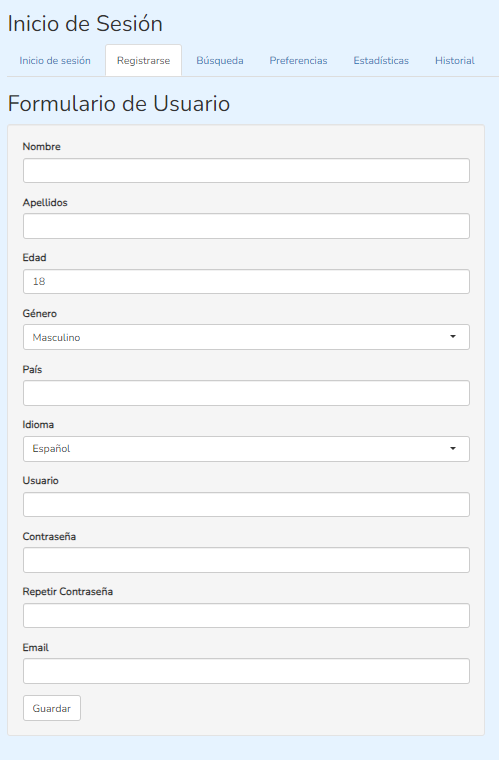
\includegraphics[width=0.5\textwidth]{imagenes/registro.png} 
        \caption{Formulario presentado al usuario}
        \label{fig:ejemplo}
    \end{figure}
    Dado que la aplicación no ha llegado a estar en explotación durante el desarrollo del trabajo, los datos que se han utilizado para trabajar con la aplicación fueron generados mediante inteligencia artificial, se le proporcionó a ChatGPT la estuctura de los datos y se le solicitaron registros falsos que siguieran esa estructura.
    \begin{figure}
        \centering
        \includegraphics[width=0.5\textwidth]{imagenes/creacionbbdd.png} 
        \caption{Respuesta ChatGPT al solicitar datos sintéticos para la base de datos}
        \label{fig:ejemplo}
    \end{figure}

    La estructura interna de la base de datos se detalla en el Anexo I apéndice C, en el manual del programador.
    \item \textbf{Preferencias}: En cuanto a las preferencias del usuario, estas se establecen mediante un formulario donde se hace una muestra de los diferentes tipos de vídeos ASMR y el usuario marca cada \textit{trigger}, de la manera marcada en la siguiente imagen, en función de si le gusta, no o si le resulta indiferente. 
    \begin{figure}
        \centering
        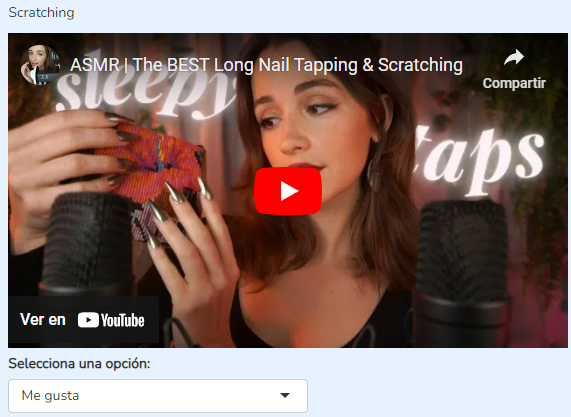
\includegraphics[width=0.5\textwidth]{imagenes/ejemplo_preferencias.png} 
        \caption{Ejemplo de selección de preferencias}
        \label{fig:ejemplo}
    \end{figure}
    Con esta misma estructura se registran las preferencias del usuario sobre los 10 tipos principales de ASMR, descritos en el apartado  3.2, subapartado \textit{Tipos de desencadenantes}. Estos datos se han introducido de manera manual durante las pruebas de uso de la aplicación, y son en los que se basan las búsquedas, excluyendo o dando preferencia a ciertas etiquetas.

    \item \textbf{Registro de sueño}: El último registro de datos proporcionado por el usuario se refiere a su calidad de sueño durante la noche anterior. Estos datos están destinados a ser estudiados posteriormente para analizar cómo ciertos tipos de videos afectan la calidad del sueño del usuario. Aunque la validez médica de estos datos es menor que si se hubieran recopilado mediante sensores en un entorno clínico, la autoevaluación sigue siendo una parte importante del proceso. En este apartado se registran los apartados más relevantes del autoreporte a la hora de la evaluación clínica: Horas de sueño, número de despertares y sensación al despertar. Los datos de este apartado se han recogido de manera mixta, por una parte se han generado datos de meses para un usuario concreto mediante inteligencia artificial y por otro se han introducido de manera manual en la aplicación.
    \begin{figure}
        \centering
        \includegraphics[width=0.3\textwidth]{imagenes/sueño_cuestionario.png} 
        \caption{Imagen del cuestionario al usuario sobre el sueño de la noche anterior}
        \label{fig:ejemplo}
    \end{figure}
    
\end{itemize}
\subsection{Datos de los vídeos}

Los datos relacionados con los vídeos se han obtenido directamente de YouTube, mediante Youtube Data API. Esta API se conecta mediante el paquete de R \textit{tuber}. Este paquete tiene múltiples funciones, de las cuales las dos más utilizadas han sido 
\begin{figure}
        \centering
        \includegraphics[width=0.5\textwidth]{imagenes/youtube data api.png} 
        \caption{Imagen Youtube Data API \cite{google}}
        \label{fig:ejemplo}
    \end{figure}

\begin{itemize}
    \item \textbf{yt search}, que realiza la búsqueda como si se estuviera utilizando directamente la aplicación de YouTube, los datos que obtiene son : El ID (que es único), la descripción, el momento de publicación, el ID del canal que lo ha publicado, las etiquetas, el enlace a las miniaturas y el tipo de resultado (video, canal o lista de reproducción). De estos datos unicamente se muestran al usuario el nombre del video, las etiquetas y el enlace, dado que se considera que el resto de parámetros, si bien es interesante almacenarlos de manera interna, no aportan información relevante para el usuario.
    \item \textbf{get stats}, esta función se aplica en el uso interno de la aplicación, los datos obtenidos no se proporcionan al usuario, son 6: id, número de visualizaciones, número de me gusta \textit{likes}, número de no me gusta \textit{dislikes}, número de favoritos (esta métrica es nula dado que con las últimas actualizaciones de YouTube no es un dato público actualmente) y número de comentarios. Estos parámetros es interesante almacenarlos para estudiar las estadísticas de popularidad de los videos que mejor funcionen a los usuarios, y tener en cuenta los resultados para optimizar las recomendaciones de la búsqueda.
    \begin{figure}
        \centering
        \includegraphics[width=0.5\textwidth]{imagenes/get_stats.jpg} 
        \caption{Muestra datos obtenidos con una búsqueda por canal con get stats}
        \label{fig:ejemplo}
    \end{figure}

\end{itemize}




\chapter{Resultados}
\section{Resumen de resultados}
\subsection{Potencial clínico}
Si bien el ASMR aún se encuentra en sus primeras etapas de investigación científica, se ha observado que tiene el potencial de ser beneficioso en una variedad de contextos clínicos. Algunas de las áreas donde el ASMR se está estudiando y mostrando resultados prometedores incluyen:
\begin{itemize}
    \item \textbf{Insomnio}: El ASMR se está estudiando en cuanto a su potencial de tratamiento de pacientes con insomnio, por su capacidad de inducir relajación en el espectador de vídeos de este tipo \cite{smejka-2022}.
    \item Manejo del dolor: Estudios recientes han explorado la capacidad de este fenómeno en el alivio de la percepción del dolor \cite{mcerlean-2022}.
    \item Ansiedad y depresión: El ASMR puede ayudar a reducir los síntomas de ansiedad y depresión, promoviendo la relajación y la liberación de endorfinas \cite{sakurai-2023}.
    \item Trastornos del espectro autista: El ASMR puede ser beneficioso para las personas con trastornos del espectro autista, ayudándolas a reducir la ansiedad, mejorar la atención y la comunicación\cite{galante-2019}.
    \item Trastorno por estrés postraumático (TEPT): Los estudios de tratamiento de pacientes con ASMR se encuentran aún en fases muy preliminares, pero parece que podría utilizarse en este campo \cite{rouw-2017}.
    \item Adicciones: El ASMR se está estudiando como un potencial tratamiento complementario para las adicciones, ayudando a reducir los antojos y la ansiedad por el sindrome de abstinencia que produce la drogadicción\cite{hu-2022}.

\end{itemize}
Es necesario destacar que la investigación sobre el ASMR aún está en curso y se necesita más investigación para confirmar plenamente sus beneficios clínicos. Sin embargo, los resultados preliminares son prometedores y sugieren que el ASMR podría ser una herramienta clínica valiosa en el tratamiento de una variedad de condiciones. La mayoría de estudios resaltan la importancia de que en caso de estar utilizando el ASMR no solamente de manera recreativa, si no como tratamiento de alguna condición o patología, este uso debería estar monitorizado y seguido por un profesional sanitario.

\subsection{Descripción del fenómeno ASMR} La Respuesta Sensorial Meridiana Autónoma es un fenómeno que produce una sensación de hormigueo o cosquilleo en la nuca, el cuero cabelludo y la espalda y una sensación de tranquilidad y relajación. Esta sensación la producen diferentes estímulos relacionados con movimientos lentos, repetitivos y sonidos suaves. Los estudios relacionados surgen en ls últimos 10 años, por lo que son relativamente recientes. La popularidad del fenómeno ha aumentado por los vídeos en redes sociales como YouTube, Instagram, TikTok o audios en Spotify. Algunos de los estímulos más populares son los susurros, toques ligeros, movimientos de manos, simulación de contacto físico, atención personal, papel, luces, comida, masajes o sonidos de la naturaleza.
\subsection{Conductas saludables y sueño} Las conductas saludables de sueño, o medidas de higiene del sueño que se recomiendan en consultas del departamento de Neurología del HUBU, que se basan en las recomendaciones generales de las organizaciones sanitarias nacionales e internacionales se pueden dividir en 6 pautas sencillas:
\begin{enumerate}
    \item Mantener horarios de sueño regulares, tanto entre semana como los fines de semana, con especial importancia en conservar una hora de despertar similar
    \item Evitar el uso de pantallas y dispositivos electrónicos durante las 2 horas previas a ir a dormir
    \item Evitar en lo posible las siestas durante el día, en caso de ser necesarias limitarlas a un máximo de 20 minutos
    \item Realizar ejercicio físico durante el día, de intensidad adecuada para el paciente, las condiciones óptimas son 1 hora, al sol y por la tarde; pero no en las 3 horas anteriores a ir a dormir, por su efecto estimulante.
    \item Eliminar (o en su defecto reducir) el uso de sustancias que puedan interferir con el sueño como son la cafeína, la nicotina o el alcohol; especialmente después de las 17:00 de la tarde.
    \item Realizar cenas ligeras unas 2 horas o 2 horas y media antes de ir a dormir, evitando tanto alimentos pesados como ayuno o ir a la cama con hambre, puesto que esto tampoco resulta positivo
\end{enumerate}
\subsection{Solución Tecnológica}
Dentro de las tecnologías utilizadas para la gestión clínica de patologías, las redes sociales son una rama muy poco explorada aún, puesto que por ahora la mayoría de estudios se centran en cómo afecta su uso tal y como es, y no en el potencial que podrían tener, y aquellos que estudian el potencial de las redes sociales, es para explorar su capacidad de divulgación \cite{diariofarma-2019}.\\*\\* Es por eso que en este trabajo se plantea la posibilidad de utilizar vídeos de YouTube, una plataforma cuya importancia social se ha descrito en el apartado 3.3, para el tratamiento del insomnio. En concreto la solución tecnológica planteada se basa en ayudar a los pacientes a relajarse y conciliar el sueño aprovechando los efectos de este tipo de vídeos tan popular. Es bajo esta premisa como se ha desarrollado la aplicación descrita a continuación.
\subsection{Aplicación Desarrollada}
La solución tecnológica que propone este trabajo es la aplicación realizada, \textit{ASMR Sleep}. \begin{figure}
    \centering
    \includegraphics[width=0.75\textwidth]{imagenes/ASMR Sleep.png}
    \caption{Logo de la aplicación}
    \label{fig:enter-label}
\end{figure}
La función de esta aplicación es facilitar el uso del ASMR a los pacientes de insomnio de conciliación, aunque también podría ser utilizada por el público general por su sencillez. Esta aplicación tiene funciones básicas para el usuario,
\begin{itemize}
    \item Configuración de preferencias basada en muestras de los tipos de vídeos más comunes de ASMR para valorar los gustos del usuario
    \item Función de búsqueda configurada para priorizar los vídeos que incluyen los estímulos favoritos del usuario y no mostrar aquellos que ha marcado negativamente
    \item Registro de datos sobre los vídeos vistos y marcados como favoritos, para facilitar el acceso posterior
    \item  Opción de autovaloración diaria en la que el usuario introduce sus sensaciones al despertar, para evaluar cómo afecta el uso de los vídeos a su calidad de sueño, pudiendo visualizar los datos recogidos y revisarlos con su médico para estudiar el proceso y evolución
\end{itemize}

\subsection{Diferenciación de roles}
\subsubsection{Usuario}
El usuario de la aplicación es el centro del desarrollo, casi todas las funciones descritas en el apartado anterior están planteadas para el usuario, que se plantea que sea un paciente de insomnio de conciliación con bajo conocimiento del ASMR, que comienza a utilizar la aplicación referido por su médico como terapia o medida complementaria al tratamiento. Dada la extensión de esta patología no se restringe el diseño en base a una demografía concreta (puede variar en edad, género, país...) al no estar limitado, se ha optado por un diseño sencillo fácil para cualquier tipo de usuario, con todas las pestañas siendo de fácil acceso y utilización intuitiva.
\begin{figure}
    \centering
    \includegraphics[width=0.75\textwidth]{imagenes/inicio de sesion.jpg}
    \caption{Inicio de la aplicación vista desde el usuario. Pestaña de inicio de sesión}
    \label{fig:enter-label}
\end{figure}

\subsubsection{Administrador}
El administrador de la aplicación tiene las funciones básicas conocidas como CRUD, por las siglas en inglés \textit{Create, Read, Update, Delete}, que corresponden a:
\begin{figure}
    \centering
    \includegraphics[width=0.75\textwidth]{imagenes/admin.png}
    \caption{Vista del administrador}
    \label{fig:enter-label}
\end{figure}
\begin{enumerate}
    \item \textbf{Crear}: Esta función muestra un registro similar al presente en la interfaz diseñada para el usuario, el administrador no tiene las limitaciones (desplegables etc.) que se ponen al usuario, por un lado debido a la capacidad de gestión y conocimiento informático que se le supone al administrador y, además, para permitir mayor libertad a la hora de realizar pruebas.
    \item \textbf{Leer}: Al introducir el email, parámetro escogido como identificador único, del usuario seleccionado, la aplicación muestra al administrador todos los datos relativos al mismo.
    \item \textbf{Actualizar}: La función de actualización permite, de nuevo, en base al email introducido, modificar uno o varios campos relativos a un usuario.
    \item \textbf{Borrar}: Previa visualización del usuario y con segundo botón de confirmación, se permite al administrador que elimine el registro relativo a un usuario.
\end{enumerate}

Además. el administrador tiene una visualización de la tabla completa de usuarios registrados en la aplicación.
\subsection{Base de datos}
Para la creación y gestión de la base de datos se ha optado por SQL, como ya se ha descrito en el apartado 4.2, la información técnica sobre la base de datos se encuentra en el Anexo I. Los conceptos generales sobre esta base de datos son la descripción de las 4 tablas que han sido utilizadas y la relación entre ellas.
\begin{enumerate}
    \item Usuarios: Esta tabla almacena los datos relativos a la información personal de los usuarios, se obtiene en el cuestionario inicial y solo puede ser modificada por el administrador
    \item Preferencias: La tabla de preferencias incluye los 10 \textit{triggers}, o estimulos, escogidos para que el usuario los valore, y en cada una de las categorías el usuario puede escoger tres valores distintos, positivo, negativo o neutral, y es ese valor escogido el que se almacena para cada estímulo. Los regstros dependen del email del usuario y pueden ser modificados en cualquier momento desde la aplicación por el usuario
    \item Estadísticas: Es una tabla que almacena para los usuarios la información sobre como han dormido la noche anterior, la pestaña de autovaloración, el usuario puede añadir 1 registro al día y no pueden eliminarse los de días anteriores puesto que se utilizan para graficar el progreso
    \item Vídeos favoritos: Los datos se obtienen directamente desde YouTube al seleccionar los vídeos desde la aplicación, y se almacena el email del usuario, el identificador de YouTube, la url, las etiquetas del vídeo seleccionado y el nombre del vídeo. Se puede almacenar un máximo de 10 vídeos por usuario y el mismo puede modificar la lista en cualquier momento.
    \begin{figure}
        \centering
        \includegraphics[width=0.5\textwidth]{imagenes/bbddsqlite.png}
        \caption{Captura de las tablas de la base de datos vista desde el gestor}
        \label{fig:enter-label}
    \end{figure}
\end{enumerate}

\subsection{Conexión API} 
La API utilizada, YouTube Data API, tiene detallada su utilización con R mediante el paquete \textit{tuber}, como ya se ha explicado anteriormente. Para utilizar esta API de manera segura, es necesario que las aplicaciones se autentiquen y obtengan el consentimiento del usuario. Este proceso de autenticación se realiza mediante OAuth 2.0, un protocolo estándar para la autorización segura. Los pasos básicos seguidos son los siguientes:
\begin{enumerate}
    \item El primer paso es crear un proyecto en Google Console, detallando nombre y propósito, para comenzar a trabajar con la conexión a la API.
    \item Una vez establecido el proyecto, es necesario buscar en la biblioteca de APIs proporcionada por Google las relativas a YouTube, para seleccionar la deseada (Data API) y habilitarla.
    \item Confiuración de consentimiento OAuth, se configura la pantalla que se mostrará a los usuarios al conectarse con su cuenta de Google se les muestra la información básica sobre la aplicación, los permisos que se solicitan detallando a qué datos concretos se quiere acceder, divididos en sensibles, no sensibles y restringidos y los usuarios de prueba (que pueden ser un máximo de 100).
    \begin{figure}
    \centering
    \includegraphics[width=0.5\textwidth]{imagenes/consentimiento OAuth.png}
    \caption{Ejemplo consentimiento cuenta de Google}
    \label{fig:enter-label}
\end{figure}
    \item Posteriormente se procede a crear unas credenciales, un ID de cliente que depende del tipo de aplicación que se esté desarrollando (en este caso una aplicación de escritorio) y se proporciona las URIs de redireccionamiento necesarias.
    \item Por último se pocede a obtener, desde los clientes de prueba creados, credenciales (ID de cliente y secreto de cliente) para poder establecer desde el código las conexiones correspondientes de manera segura mediante la función \textbf{yt auth}.
\end{enumerate}
La ventaja que presenta esta conexión es el acceso a la información sobre las consultas que se ejecutan, en la imagen 5.6 se observa el número de consultas y sus estadísticas en el periodo entre el 5 de mayo de 2024 y el 5 de junio de 2024, en las fases finales de desarrollo de la aplicación y en la fase de pruebas.
\begin{figure}
    \centering
    \includegraphics[width=1\textwidth]{imagenes/consultas_mayo_junio.png}
    \caption{Consultas 05.05.2024 a 05.06.2024}
    \label{fig:enter-label}
\end{figure}

\subsection{Frontend en CSS}
El frontend de una aplicación define la estética y la experiencia visual de la interfaz de usuario, incluyendo la elección de fuentes, colores, y disposición de elementos.

En el desarrollo del frontend de la aplicación realizada en Shiny desde RStudio, uno de los objetivos fue el diseño de una interfaz atractiva y funcional. Para lograr esto, se creó un archivo `estilo.css` que define los estilos visuales de la aplicación. Este archivo CSS incluye la importación de la fuente 'Nunito' desde Google Fonts, proporcionando una apariencia moderna y agradable. Además, se establecen propiedades de diseño para el cuerpo de la página, tales como un color de fondo azul suave, un color comunmente relacionado con el sueño, y un ajuste óptimo de la imagen de fondo. 

También se diseñaron componentes específicos como el contenedor de inicio de sesión (`.login-container`), que presenta una estructura limpia y centrada, con un borde redondeado y un fondo blanco para resaltar los elementos dentro de él. La clase `.login-title` se estilizó para que el título de la sección de inicio de sesión sea prominente, con un tamaño de fuente significativo y un color que garantiza una buena legibilidad. Este enfoque de diseño contribuyó a una experiencia de usuario sencilla y cohesiva dentro de la aplicación. Se puede observar el resultado en la imagen 5.2.

\subsection{Mejoras futuras}
En este apartado se van a explorar cuales podrían ser posibles mejoras futuras para la aplicación, para tenerlas en cuenta en actualizaciones posteriores.
\begin{enumerate}
    \item En primer lugar, los tiempos de espera de la aplicación son demasiado grandes, debido a que la conexión con YouTube desde Google Cloud se realiza desde una versión gratuita de prueba, con la aplicación en explotación se podría buscar la manera de financiar una versión con más posibilidades, que aceleraran las búsquedas.
    \item La aplicación tiene unas medidas de seguridad poco desarrolladas, se podrían implementar medidas como sugerencia de contraseñas seguras, utilizar un doble factor de autenticación, encriptar la base de datos donde están almacenadas, guardar el secreto de cliente en un servidor apartado al que se acceda desde el código de aplicación.
    \item Al almacenar las etiquetas de aquellos videos que los usuarios marcan como favoritos se podría hacer un análisis de tendencias en función de las características de los usuarios, creando un algoritmo inteligente de recomendación, \textit{wordclouds} o nubes de palabras de las búsquedas comunes del usuario, mapas de tendencias por países, entre otras opciones que ofrece Shiny.
    \item Pese a que la aplicación está planteada enteramente en castellano, podría ofrecerse la posibilidad de traducirla a otros idiomas.
    \item El enfoque inicial de esta aplicación ha sido como una aplicación web, en futuras actualizaciones se podría ofrecer una versión móvil de la misma.
    \item  Dada la constante mejora en la fiabilidad de los datos registrados por los relojes inteligentes, no solo se podría recomendar a los usuarios que contrasten sus respuestas de la pestaña de estadísticas con lo que marquen sus relojes, en caso de tenerlos, si no que también se podría plantear la posibilidad de que se conecte directamente con la aplicación para volcar los datos.
\end{enumerate}

\chapter{Conclusiones}
En este trabajo, se ha explorado el fenómeno del ASMR como una herramienta popular pero aún insuficientemente estudiada en el ámbito clínico. A pesar de su amplia aceptación entre los usuarios de Internet, su potencial terapéutico permanece en gran medida sin explotar, lo que destaca la necesidad urgente de investigaciones más rigurosas y específicas que puedan evaluar su efectividad y posibles aplicaciones en el tratamiento de diversos trastornos de salud mental y física. Paralelamente, se ha observado cómo las redes sociales han adquirido una posición de influencia significativa en el ámbito sanitario, brindando oportunidades para la difusión de información médica, el apoyo a pacientes y la colaboración entre profesionales de la salud. Este fenómeno plantea desafíos y oportunidades, sugiriendo la necesidad de un enfoque crítico y ético para aprovechar su potencial al máximo en beneficio de la salud pública.

Además, en un contexto marcado por el aumento en el uso de aplicaciones móviles y tecnología digital en la atención médica y la gestión de la salud, se destaca la importancia de que los ingenieros de la salud desarrollen competencias en el diseño y la implementación de estas herramientas. Este conocimiento no solo garantizará la creación de aplicaciones efectivas y seguras, sino que también promoverá una colaboración más estrecha entre profesionales de la salud y expertos en tecnología, impulsando así la innovación y la mejora continua en la atención médica. En resumen, este trabajo subraya la necesidad de aprovechar el potencial de la tecnología y las redes sociales de manera ética y reflexiva, reconociendo su papel fundamental como medio de intervención en la promoción de la salud y el bienestar en la sociedad contemporánea.

\chapter{Líneas de trabajo futuras}
Las líneas de trabajo futuras, desde el punto de vista de la aplicación desarrollada se encuentran en el punto 5.1, en mejoras futuras, y en cuanto a la investigacion sobre el ASMR, hay 5 puntos principales que se pueden plantear para futuros estudios:
\begin{enumerate}
    \item Efectividad terapéutica: Investigaciones más rigurosas podrían examinar de manera más detallada la efectividad del ASMR como herramienta terapéutica en el tratamiento de trastornos específicos, como el estrés, la ansiedad, el insomnio o el dolor crónico. Estudios controlados y aleatorizados podrían comparar el ASMR con otras intervenciones terapéuticas convencionales para determinar su eficacia relativa.
    \item Mecanismos neurológicos: Explorar los mecanismos neurológicos y reacciones fisiológicas subyacentes al ASMR es crucial para comprender cómo y por qué esta experiencia induce sensaciones placenteras y efectos calmantes en algunas personas. Investigaciones con técnicas de neuroimagen funcional podrían identificar las regiones cerebrales involucradas y los neurotransmisores implicados en la respuesta al ASMR.
    \item Variedad de estímulos: Dado que el ASMR puede ser desencadenado por una variedad de estímulos sensoriales, como susurros, sonidos suaves, movimientos lentos y toques suaves, sería importante investigar cómo diferentes tipos de estímulos afectan la experiencia del ASMR y su potencial terapéutico.
    \item Perfil de los receptores: Explorar las características individuales que influyen en la sensibilidad al ASMR, como la personalidad, la sensibilidad sensorial y las experiencias previas, puede ayudar a identificar quiénes son más propensos a beneficiarse de las intervenciones basadas en el ASMR.
    \item Aplicaciones clínicas: Una vez que se haya establecido la efectividad del ASMR como herramienta terapéutica, se podrían desarrollar y evaluar intervenciones específicas basadas en el ASMR para una variedad de problemas de salud mental y física, adaptadas a las necesidades individuales de los pacientes.

\end{enumerate}
En conjunto, estas líneas de investigación podrían contribuir significativamente al entendimiento del ASMR y su potencial como una herramienta clínica efectiva en el futuro.

\bibliographystyle{apalike}
\bibliography{bibliografia}

\end{document}
